
%%%%%%%%%%%%%%%%%%%%%%% file typeinst.tex %%%%%%%%%%%%%%%%%%%%%%%%%
%
% This is the LaTeX source for the instructions to authors using
% the LaTeX document class 'llncs.cls' for contributions to
% the Lecture Notes in Computer Sciences series.
% http://www.springer.com/lncs       Springer Heidelberg 2006/05/04
%
% It may be used as a template for your own input - copy it
% to a new file with a new name and use it as the basis
% for your article.
%
% NB: the document class 'llncs' has its own and detailed documentation, see
% ftp://ftp.springer.de/data/pubftp/pub/tex/latex/llncs/latex2e/llncsdoc.pdf
%
%%%%%%%%%%%%%%%%%%%%%%%%%%%%%%%%%%%%%%%%%%%%%%%%%%%%%%%%%%%%%%%%%%%


\documentclass[runningheads,a4paper]{llncs}

\usepackage{amssymb}
\usepackage{amsmath}
\setcounter{tocdepth}{3}
\usepackage{graphicx}
\newtheorem{mydef}{Definition}
\newtheorem{mylemma}{Lemma}
\usepackage{algorithm}
\usepackage[noend]{algpseudocode}


\usepackage{url}
\urldef{\mailsa}\path|{jayg, cmhill, mpop}@cs.umd.edu|    
\newcommand{\keywords}[1]{\par\addvspace\baselineskip
\noindent\keywordname\enspace\ignorespaces#1}

\begin{document}

\mainmatter  % start of an individual contribution

% first the title is needed
\title{Identifying Inter-Genomic Repeats Using Fast, Approximate Methods for Betweenness Centrality}

% a short form should be given in case it is too long for the running head
\titlerunning{Inter-Genomic Repeats Using Betweenness Centrality}

% the name(s) of the author(s) follow(s) next
%
% NB: Chinese authors should write their first names(s) in front of
% their surnames. This ensures that the names appear correctly in
% the running heads and the author index.
%
\author{Jay Ghurye%
\and Christopher M. Hill\and Mihai Pop}
%
\authorrunning{Ghurye et al.}
% (feature abused for this document to repeat the title also on left hand pages)

% the affiliations are given next; don't give your e-mail address
% unless you accept that it will be published
\institute{University of Maryland, College Park\\
\mailsa\\}

%
% NB: a more complex sample for affiliations and the mapping to the
% corresponding authors can be found in the file "llncs.dem"
% (search for the string "\mainmatter" where a contribution starts).
% "llncs.dem" accompanies the document class "llncs.cls".
%

\toctitle{Lecture Notes in Computer Science}
\tocauthor{Authors' Instructions}
\maketitle


\begin{abstract}
Assembling metagenomic data is a challenging task due to several reasons. One of the reasons that complicates assembly is the sequences shared between the genomes of multiple organisms. Such regions in genomes are called repeats. Repeats make assembly difficult because they link the unrelated sections of genomes. It has been shown that the number of reconstructions of genome grows exponentially with repeats. Existing approaches to identify repeats are inefficient and do not scale well as size of data increases. We propose an application of a core concept in social network analysis called betweenness centrality to metagenomic data to identify inter-genomic repeats. We study how approximation algorithms for betweenness centrality can be useful to find central nodes quickly and propose a novel approach to identify inter-genomic repeats accurately. 
\keywords{Metagenomics, Algorithms, Centrality, Graph}
\end{abstract}


\section{Introduction}

Metagenomic data are considerably more complex. The assembly of metagenomic data is complicated due to several reasons. Few of them are: (i) widely different levels of representation for different organisms in a community; (ii) genomic variation between closely related organisms; (iii) conserved genomic regions shared by distantly related organims; and (iv) repetitive sequences within individual genomes. Genomic repeats are the major challenge when assembling isolated genomes and their effect is prominently seen in metagenomic datasets. It has been shown by Kingsford et al.\cite{kingsford} that the number of reconstructions grow exponentially with the number of repeats. Therefore it is impossible find one correct solution for assembly. There are several approaches such as \cite{bambus} to find repeats in metagenomic data. The main drawback of these methods is that they do not scale well as number of nodes in assembly graph increase and prove very inefficient as number of nodes reaches to about a million. To tackle this problem, we explore some of the work in social network analysis, particularly in the area of node centrality. We make use of betweenness centrality to find out repeats in assembly graph. 

\section{Related Work}

\subsection*{Betweenness Centrality}
In graph theory and network analysis, indicators of centrality identify the most important vertices within a graph.Several metrics to measure centrality have been proposed. We make use of betweenness centrality. For a particular node, betweenness centrality is equal to the number of shortest paths from all vertices to all others that pass through that node. Formally, for a node $v$, it is defined by following expression:

$$g(v) = \sum_{s \neq t \neq v} \frac{\sigma_{st}(v)}{\sigma_{st}}$$

where $\sigma_{st}$ is the total number of shortest paths from node $s$ to node $t$ and $\sigma_{st}(v)$ is the number of those paths passing through $v$.

Brandes\cite{brandes} gives an exact algorithm for computing betweenness centrality of all the nodes that is based on solving a single source shortest path problem for each node. An SSSP computation from $s$ produces a directed acyclic graph (DAG) encoding all shortest paths starting at $s$. By backward aggregation of counter values, the contributions of these paths to the betweenness counters can be computed in linear time. Brandes algorithm explains how to calculate $\sigma_{st}$ on the fly during shortest path calculations: $\sigma_{ss} = 1$ and for $s \neq t, \sigma_{st} = \sum_{v \in pred(t)} \sigma_{sv}$ where $pred(t)$ is a multiset containing the immediate predecessors of  $t$ in the shortest path DAG. In a subsequent aggregation phase, the nodes are processed in reverse topological order, i.e. by non-decreasing distance from $s$. So we have: 
$$\delta_{s}(v) = \sum_{w \in succ(v)} \frac{\sigma_{sv}}{\sigma_{sw}}(1+\delta_{s}(w))$$

where $\delta_{s}(v) = \frac{\sigma_{st}(v)}{\sigma_{st}}$ and $succ(v)$ is an immediate successor of $v$  in the shortest path DAG.   
This algorithm takes time $\Theta(mn)$ for unit edge weight graphs and $\Theta(mn + n^{2}log(n))$ for weighted graphs. This algorithm does not scale well with large networks with millions of nodes and edges. Bader and Madduri\cite{bader} provide a massively parallel implementation of the exact algorithm. However this approach scales to about a few million nodes. 

\subsection*{Betweenness Centrality Based on Sampling Nodes}
Due to scalability limitations of exact betweenness centrality, several approximation algorithms for betweenness centrality have been proposed. Bader and Pich\cite{bp} provide an approximation algorithm by extrapolating from a subset of $k$ starting nodes called pivots and using same aggregation strategy as exact betweeness algorithm. However, this algorithm overestimates the centrality of some unimportant nodes which lie near pivot. The approximation algorithm proposed by Geisberger et al. \cite{sanders} comes over this drawback by changing the scheme for aggregating betweenness contributions so that nodes do not get profited just because they are near pivot. They define an estimator for betweenness centrality. This estimator is characterized by a length function $l : E \Rightarrow \mathbb{R}$ on the edges and a scaling function $f : [0,1] \Rightarrow [0,1]$. For a path $P = (e_{1},e_{2}...,e_{k})$ let $l(P) := \sum_{1 \leq i \leq k} l(e_{i})$. Let $n$ be the number of sample nodes chosen from a graph. The algorithm works as follows: In each iteration one of $2n$ shortest path searches is performed with uniform probability $1/2n$. An iteration can be a forward search in $G = (V,E)$ from a pivot $s \in V$ ($|V| = n$) or backward search from a pivot $t \in V$, that is a search from $t$ in $(V,{(v,u) : (u,v) \in E})$. For each shortest path of the form 
$$ P = (\overbrace{s,...,v}^{Q},..,t)$$ 
a scaled contribution is defined as follows:\\

\begin{equation*}
	\delta_{P}(v) := \begin{cases}
					\frac{f(l(Q)/l(P))}{\sigma_{st}} & \text{for a forward search} \\\\
					\frac{1 - f(l(Q)/l(P))}{\sigma_{st}} & \text{for a backward search} 
					\end{cases}
\end{equation*}

Overall, $v$ receives contribution 

$$\delta(v) := \delta_{s}(v) := \sum_{t \in V}\sum \{\delta_{P}(v):  P \in SP_{st}(v)\}$$
due to a forward search, and 

$$\delta(v) := \delta_{t}(v) := \sum_{s \in V}\sum \{\delta_{P}(v):  P \in SP_{st}(v)\}$$
due to a backward search. 

This algorithm is efficiently implemented using two techniques. First one is \textit{linear scaling}, where the contribution of a node $v$ depends linearly on the distance to the sample. Nearer the node is to the sample, lesser is its contribution counted. Linear scaling is implemented using a simple variant of aggregation scheme proposed in Brandes algorithm. Second technique is \textit{bisection scaling} where the sample only contributes to the second half of a path. This means that for a vertex $v$, its contribution is considered only if it is at atleast half distance between $s$ and $t$ away from $s$ in forward search or more than half a distance away from $t$ in backward search. 



\begin{figure}[htbp]
\centering
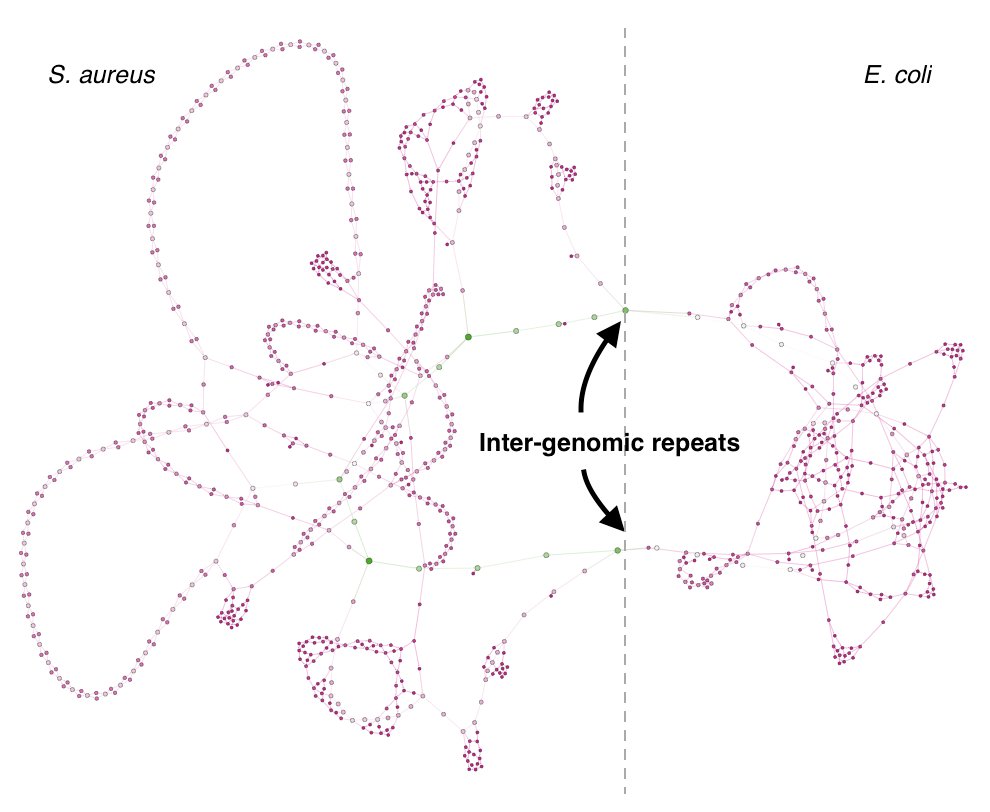
\includegraphics[width = \textwidth]{es_mix_200kb_k21.png}
\caption{Example of conversion of de Bruijn graph to Repeats graph}
\label{fig:sampled_nodes}
\end{figure}


\subsection*{Betweenness Centrality Based on Sampling Shortest Paths}
There  is another approximation algorithm was proposed by Matteo et al. \cite{matteo} based on randomized sampling of shortest paths and offer probabilistic guarantees on the quality of approximation. This algorithm guarantees that all approximate values of betweenness for all vertices are within an additive factor $\epsilon \in (0,1)$ from the real values with probability at least $1-\delta$. To derive bounds on sample size, results from VC dimension theory\cite{vc} are used. The main advantage of this algorithm is that the sample size does not depend on the size of the graph, but only on the maximum number vertices in a shortest path which is called \textit{vertex diameter}.  

The Vapnik-Chernovenkis(VC) dimensions of a class of subset is defined on a set of points is a measure of expressiveness of such class. Given a probability distribution on the set of points, a finite bound on the VC-dimension of the class of subsets implies a bound on the number of random samples required to approximate the probability of each subset in the class with its empirical average. This technique is used to derive the expressiveness of the sample of shortest paths derived. For graph $G(V,E)$, let $S_{all}$ be the union of $T_{v}$ for all $v \in V$, where $T_{v}$ is the set of all shortest path to which $v$ is internal. VC dimension technique helps in choosing sample from $S_{all}$ so that it gives probabilistic guarantees. It is shown that the upper bound on VC dimensions of $S_{all}$ is given by:
$$VC(S_{all}) \leq \left\lfloor{log_{2}(VD(G) - 2)}\right\rfloor + 1$$
where $VD(G)$ is vertex diameter of $G$. Using this upper bound, sample size $r$ can be estimated as follows:
\begin{equation} \label{sample_size_algo}
r = \frac{c}{\epsilon^{2}}(\left\lfloor{log_{2}(VD(G) - 2)}\right\rfloor + 1 + ln\frac{1}{\delta})
\end{equation} 
where $c$ is a universal constant with value $0.5$. It is guaranteed that betweenness centralities estimated using this sample size are within additive factor $\epsilon$ from real values with probability atleast $1-\delta$. 

Complete algorithm is sketched in algorithm 1. There are two crucial things in this algorithm. First is computing approximate vertex diameter. Calculating exact VD(G) will need to solve all pair shortest  path problem. The complexity of this algorithm is $O(V^{2}logV + VE)$ by Johnson's algorithm\cite{johnson} and $\Theta(V^{3})$ by Floyd-Warshall algorithm. This would be very slow. A faster linear time 2-approximation algorithm is proposed in \cite{matteo} is used to calculate approximate vertex diameter. 

Second is to sample shortest paths. They way a random shortest path from $S_{uv}$ is inspired by Brandes algorithm\cite{brandes}. Assume that $u$ and $v$ are connected. For each vertex $w$, let $P_{u}(w)$ be a subset of neighbors of $w$ which are predecessors of $w$ along the shortest path from $u$ to $w$. Let $p^{*}$ be the sampled shortest path that we build backwards starting from the endpoint $v$ and by adding sampled predecessors before $v$. Initially $p^{*} = {v}$. Starting from $v$, we select it's predecessor $z \in P_{u}(v)$ using weighted random sampling. Each $z \in P_{u}(v)$ has probability $\sigma_{uz}/\sum_{w \in P_{u}(v)}\sigma_{uv} = \sigma_{uz}/\sigma_{uv}$. We add $z$ to $p^{*}$ and repeat this procedure until $z \neq u$. In the end, we have single shortest path sampled from $S_{uv}$. 
 
\begin{algorithm}
\caption{Algorithm to compute approximate betweenness centrality}
\begin {algorithmic}[1]
\State {\textbf{Input}:Graph $G(V,E)$ with $|V| = n,\epsilon,\delta \in (0,1)$}
\State {\textbf{Output}: A set of approximate betweenness centrality for all nodes $v$ in $G$}
\For {$v \in V$}
\State {$b'(v) = 0$}
\EndFor 
\State {$VD(G) \leftarrow \mathtt{getVertexDiameter}(G)$}
\State {$r \leftarrow \frac{c}{\epsilon^{2}}(\left\lfloor{log_{2}(VD(G) - 2)}\right\rfloor + 1 + ln\frac{1}{\delta})$}
\For{$i \leftarrow 1$ to $r$}
\State {$(u,v) = \mathtt{SampleUniformVertexPair(V)}$}
\State {$S_{uv} = \mathtt{ComputeAllShortestPath(u,v)}$}
\If {$S_{uv} \neq \{p_{\phi}\}$}
\State 	{$t \leftarrow v$}
\While {$t \neq u$}
\State {sample $z \in P_{u}(t)$ with probability $\sigma_{uz}/\sigma_{ut}$}
\If {$z \neq u$}
\State {$b'(z) \leftarrow b'(z) + 1/r$}
\EndIf
\State {$t \leftarrow z$}
\EndWhile
\EndIf
\EndFor\\
\Return {$(v,b'(v)) :\forall v \in V$}
\end{algorithmic}
\end{algorithm}

Analysis of this algorithm shows that it offers probabilistic guarantees on the quality of all approximations of the betweenness centrality. Let $b(v)$ be the actual betweenness centrality of node $v$ and $b'(v)$ be the betweenness centrality returned by algorithm 1. Then following lemma holds:

\begin{mylemma}
With probability atleast $1-\delta$, all the approximations computed by the algorithm are within $\epsilon$ from their real value:
$$Pr(\exists v \in V s.t. |b(v) - b'(v)| > \epsilon) < \delta$$
\end{mylemma}

The runtime of this algorithm is dominated by the computation of shortest path at each step which takes time $O(|V| + |E|)$ if graph is unweighted (BFS) and $O(|E| + |V|log|V|)$ othewise (Dijkstra's algorithm). This is multiplied by $r$ for $r$ iterations to obtain final complexity.


\section{Methods}

\subsection*{De Bruijn Graph} 

De Bruijn strings are a type of 'comprehensive' strings. For a given alphabet $\Sigma = \{A,C,T,G\}$ and a length $k$, a de Bruijn string of order $k$ contains as substrings of length $k$ over $\Sigma$. These strings can be represented in a sophisticated way in term of a graph called de Bruijn graph \cite{debruijn}. A de Bruijn graph of order $k$ is a graph that contains all strings of length $k-1$ from a given alphabets as nodes and contains edges between two nodes if the corresponding strings overlap by exactly $k-2$ letters in prefix-suffix manner. In other words, each $k$-mer is represented by two nodes in a graph connected by an edge. 

We modify the de Bruijn graph generated from genomes to identify repeats in a better way. We define \textit{unipaths} as the path of nodes in which the outdegree of first node on the path is $1$ and indegree is greater than $1$, indegree of last node on the path is $1$ and outdegree is greater than $1$ and for all other nodes, both indegree and out degree is exactly $1$. We compress all the unipaths in a graph to represent in a compact way. For all the internal nodes on unipaths, we represent them by a single node with label as the combined label of all nodes. figure\ref{fig:repeatgraph} shows an example of such compression of unipaths in de Bruijn graphs. 

\begin{figure}[htbp]
\centering
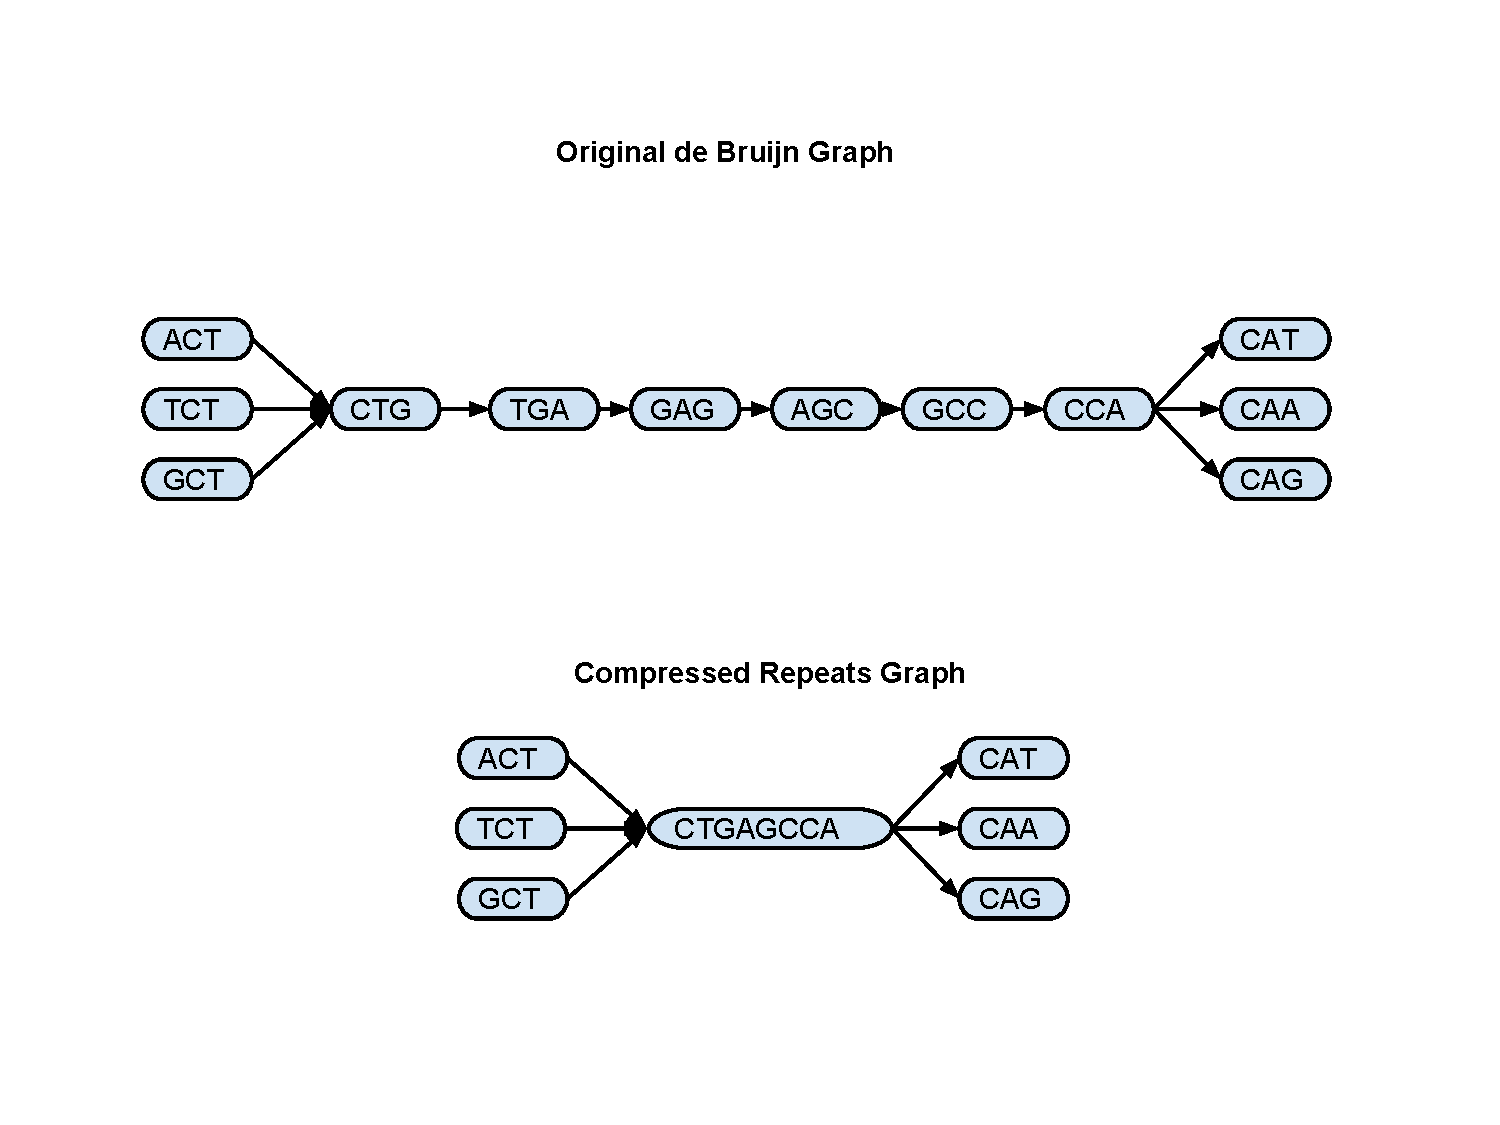
\includegraphics[width = \textwidth]{repeatgraph}
\caption{Example of conversion of de Bruijn graph to Repeats graph}
\label{fig:repeatgraph}
\end{figure}

\subsection*{Networkit}
We investigated the performance of approximate betweenness centrality algorithms on the metagenomic graphs to find inter-genome repeats. We used the implementations provided by  Networkit\cite{networkit} library. NetworKit is an open source library for high-performance network analysis. It implements effecient graph algorithms and parallelize most of them. It provides implementation for variety of centrality measures. We used the implementation of approximate betweenness centrality. NetworKit provides parallelized implementation of the algorithm by Matteo et al.\cite{matteo} which is based on sampling shortest paths. It also provides implementation for the algorithm by Geisberger et al.\cite{sanders}. However, this algorithm is not parallelized. 


\subsection*{Cutoff Criteria For Repeats}
To determine which nodes in a graph should be marked as repeats, we define a criteria based on the value of centrality calculated by the algorithm. Let $x$ be the mean of centralities of all the nodes and $\sigma$ be the standard deviation. A node $v$ is marked as repeat only if the following condition holds: $b(v) \geq x + c*\sigma$ where $c$ is a constant and $b(v)$ is betweenness centrality of the node. We set value of $c$ as 3 as it works out the best.

Another cutoff criteria we test is based on \textit{interquartile range(IQR)}. Let $Q_{1}$,$Q_{2}$, and $Q_{3}$ denote lower, middle and upper quartile respectiely. IQR can be defined as the difference between the upper and lower quartile. So, $IQR = Q_{3} - Q_{1}$. For the values of centrality, we calculate upper quartile, middle quartile, lower quartile and IQR. For filtering, we mark all the nodes with centrality more than $Q_{2} + 1.5*IQR$ as repeats. The advantage of this method is that it does not make any assumptions about the distribution of underlying data.  

\section{Results} 
We evaluated algorithms for betweenness centrality to find inter-genome repeats on real datasets described above. We use the notion of sensitivity and specificity to define the accuracy of repeat detection. A good repeat detection strategy should have both high sensitivity and specificity. Sensitivity is the measure of proportion of actual repeats which are correctly identified by the algorithm. Specificity is the proportion of non-repeats correctly identified by the algorithm. High sensitivity is desired because we want to remove as many repeats from the graph. High specificity is desired becasue we do not want to remove non-repeats which are incorrectly identified as repeats by algorithm. To calculate sensitivity and specificity, we define following terms:
\begin{itemize}
\item \textbf{True positives(TP):} Number of nodes marked as repeat that is found within at least 2 genomes
\item \textbf{False positives(FP):} Number of nodes marked as repeat that is only repetitive within a single genome
\item \textbf{True negatives(TN):} Number of nodes marked as non-repeat that is only repetitive within a single genome
\item \textbf{False negatives(FN):} Number of nodes marked as non-repeat that is found within at least 2 genomes
\end{itemize}

Using these quantities, we can define sensitivity and specificity as follows:
 $$Sensitivity = \frac{TP}{TP+FN}$$
 $$Specificity = \frac{TN}{TN+FP}$$


\begin{figure}[htbp]
\centering
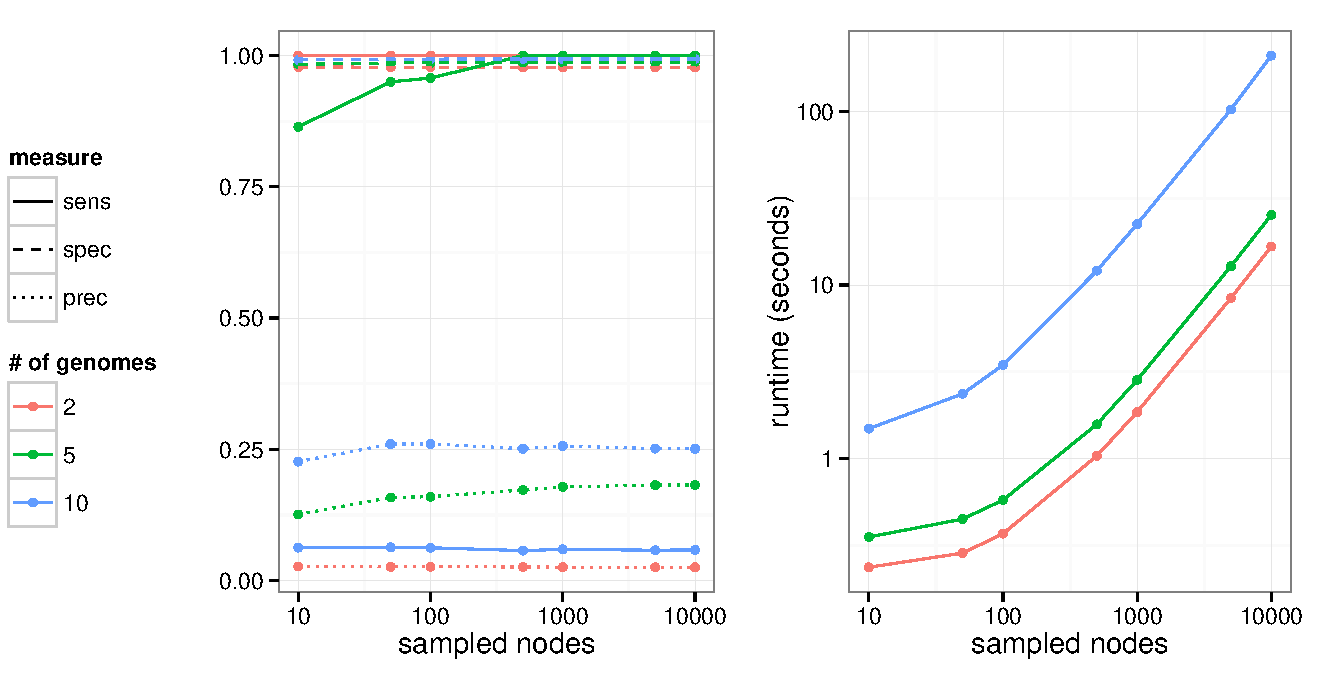
\includegraphics[width = \textwidth]{sampled_nodes}
\caption{Example of conversion of de Bruijn graph to Repeats graph}
\label{fig:sampled_nodes}
\end{figure}

\begin{figure}[htbp]
\centering
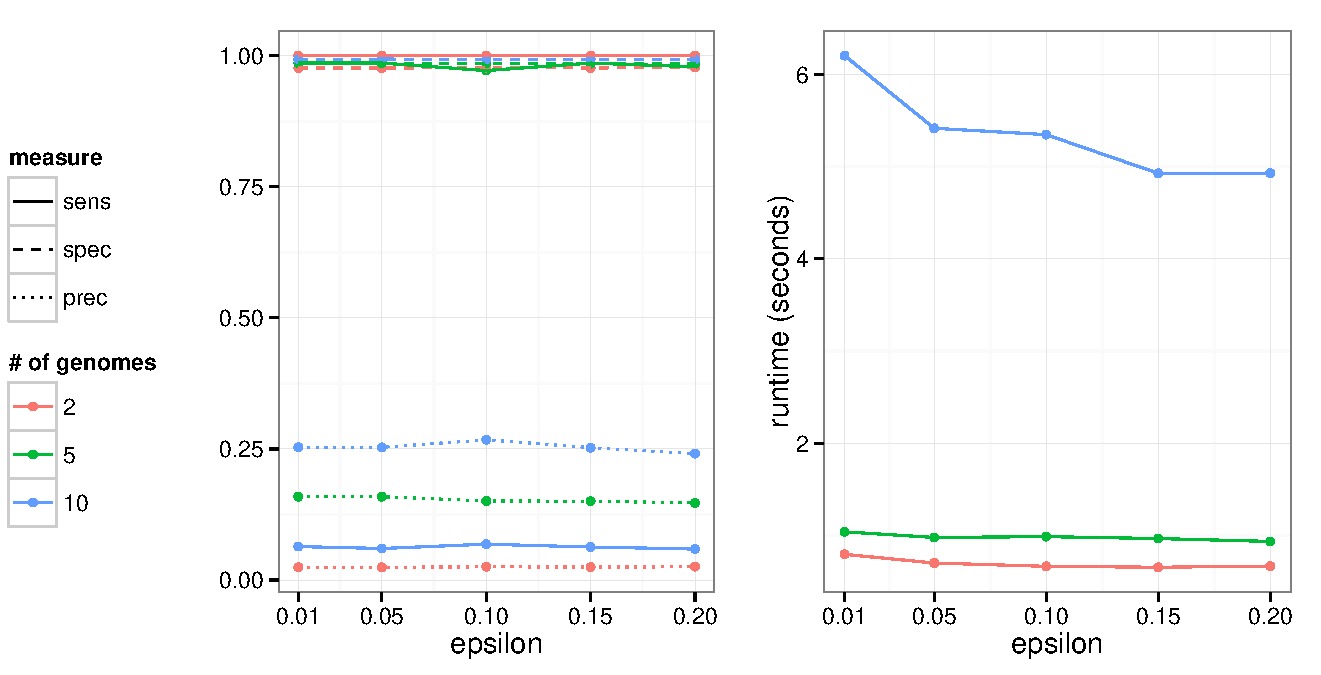
\includegraphics[width = \textwidth]{sampled_paths}
\caption{Example of conversion of de Bruijn graph to Repeats graph}
\label{fig:sampled_nodes}
\end{figure}

\section{Conclusion}
In this work, we show how approximate betweenness centrality can be used to identify inter-genome repeats. We explored two algorithms, one based on sampling shortest paths in a graph and other based on sampling nodes in a graph. Application of both these algorithms to repeat detection problem provided significantly accurate and fast results. We explore how various parameters such as number of sampled nodes and filtering criteria to mark a node as repeat affects the accuracy of repeat detection. We are planning to use these techniques for repeat detection in our future metagenomic assembler. 
\bibliography{manuscript}{}
\bibliographystyle{abbrv}

\end{document}
